%%%%%%%%%%%%%%%%%%%%%%%%%%%%%%%%%%%%%%%%%
% baposter Landscape Poster
% LaTeX Template
% Version 1.0 (11/06/13)
%
% baposter Class Created by:
% Brian Amberg (baposter@brian-amberg.de)
%
% This template has been downloaded from:
% http://www.LaTeXTemplates.com
%
% License:
% CC BY-NC-SA 3.0 (http://creativecommons.org/licenses/by-nc-sa/3.0/)
%
%%%%%%%%%%%%%%%%%%%%%%%%%%%%%%%%%%%%%%%%%

%----------------------------------------------------------------------------------------
%	PACKAGES AND OTHER DOCUMENT CONFIGURATIONS
%----------------------------------------------------------------------------------------

\documentclass[landscape,archE1,fontscale=0.315]{baposter} % Adjust the font scale/size here

\usepackage{graphicx} % Required for including images
\graphicspath{{figures/}} % Directory in which figures are stored

\usepackage{amsmath} % For typesetting math
\usepackage{amssymb} % Adds new symbols to be used in math mode

\usepackage{booktabs} % Top and bottom rules for tables
\usepackage{enumitem} % Used to reduce itemize/enumerate spacing
\usepackage{palatino} % Use the Palatino font
\usepackage[font=small,labelfont=bf]{caption} % Required for specifying captions to tables and figures

\usepackage{multicol} % Required for multiple columns
\setlength{\columnsep}{1.5em} % Slightly increase the space between columns
\setlength{\columnseprule}{0mm} % No horizontal rule between columns

\usepackage{tikz} % Required for flow chart
\usetikzlibrary{shapes,arrows} % Tikz libraries required for the flow chart in the template

\newcommand{\compresslist}{ % Define a command to reduce spacing within itemize/enumerate environments, this is used right after \begin{itemize} or \begin{enumerate}
\setlength{\itemsep}{1pt}
\setlength{\parskip}{0pt}
\setlength{\parsep}{0pt}
}

\definecolor{lightblue}{rgb}{0.145,0.6666,1} % Defines the color used for content box headers

\begin{document}

\begin{poster}
{
headerborder=closed, % Adds a border around the header of content boxes
colspacing=1em, % Column spacing
bgColorOne=white, % Background color for the gradient on the left side of the poster
bgColorTwo=white, % Background color for the gradient on the right side of the poster
borderColor=lightblue, % Border color
headerColorOne=black, % Background color for the header in the content boxes (left side)
headerColorTwo=lightblue, % Background color for the header in the content boxes (right side)
headerFontColor=white, % Text color for the header text in the content boxes
boxColorOne=white, % Background color of the content boxes
textborder=roundedleft, % Format of the border around content boxes, can be: none, bars, coils, triangles, rectangle, rounded, roundedsmall, roundedright or faded
eyecatcher=true, % Set to false for ignoring the left logo in the title and move the title left
headerheight=0.1\textheight, % Height of the header
headershape=roundedright, % Specify the rounded corner in the content box headers, can be: rectangle, small-rounded, roundedright, roundedleft or rounded
headerfont=\Large\bf\textsc, % Large, bold and sans serif font in the headers of content boxes
%textfont={\setlength{\parindent}{1.5em}}, % Uncomment for paragraph indentation
linewidth=2pt % Width of the border lines around content boxes
}
%----------------------------------------------------------------------------------------
%	TITLE SECTION 
%----------------------------------------------------------------------------------------
%
{
\includegraphics[height=4em]{gtcmt}} % First university/lab logo on the left
{\bf\textsc{Chord Detection Using \\ Deep Learning}\vspace{0.5em}} % Poster title
{\textsc{\{ Xinquan Zhou and Alexander Lerch \} \hspace{12pt} \\ Georgia Tech Center for Music Technology}} % Author names and institution
%{
\includegraphics[height=4em]{logo.png}} % Second university/lab logo on the right

%----------------------------------------------------------------------------------------
%	introduction
%----------------------------------------------------------------------------------------

\headerbox{Introduction}{name=objectives,column=0,row=0}{
Chord detection is to automatically
recognize the chord progression in a music recording. 
Several studies indicate that deep learning methods can be very successful
when applied to Music Information Retrieval (MIR)
tasks, especially when used for feature learning \cite{hamel2010learning}.
Deep learning, with its potential to untangle complicated
patterns in large amounts of data, should be well suited for
the task of chord detection.

%Deep architectures
%promise to remove the necessity of custom-designed
%and manually selected features as neural networks should
%be more powerful in disentangling interacting factors and
%thus be able to create meaningful high-level representations
%of the input data.
%\begin{enumerate}\compresslist
%\item Feugiat vitae elit
%\item bibendum ante sed lacinia eros in
%\item Curabitur scelerisque arcu consequat varius
%\item Dapibus nulla id purus consectetur
%\item Fringilla integer 
%\end{enumerate}

\vspace{0.3em} % When there are two boxes, some whitespace may need to be added if the one on the right has more content
}

%----------------------------------------------------------------------------------------
%	data set
%----------------------------------------------------------------------------------------

\headerbox{Data set}{name=dataset,below=objectives,column=0}{

%Aliquam non lacus dolor, \textit{a aliquam quam}. Cum sociis natoque penatibus et magnis dis parturient montes, nascetur ridiculus mus. Nulla in nibh mauris. Donec vel ligula nisi, a lacinia arcu. Sed mi dui, malesuada vel consectetur et, egestas porta nisi. Sed eleifend pharetra dolor, et dapibus est vulputate eu. \textbf{Integer faucibus elementum felis vitae fringilla.} In hac habitasse platea dictumst. Duis tristique rutrum nisl, nec vulputate elit porta ut. Donec sodales sollicitudin turpis sed convallis. Etiam mauris ligula, blandit adipiscing condimentum eu, dapibus pellentesque risus.
%
Our data set is a 317-piece collection:
\begin{itemize}\compresslist
  \item 180 songs from the Beatles dataset
  \item 100 songs from the RWC Pop dataset
  \item 18 songs from the Zweieck dataset and
  \item 19 songs from Queen dataset
\end{itemize}
The target chords are major and minor triads for every root note plus one none class resulting in 25 (12+12+1) chord labels. Ground truth time-aligned chord symbols are mapped into the major/minor dictionary:
\begin{equation*}
Chord_{majmin} \subset \{N\} \cup \{S \times {maj,min}\}
\end{equation*}
Triad major/minor and seventh major/minor are mapped into the corresponding major/minor label. Other chord
types are treated as unknown chords.
\begin{center}
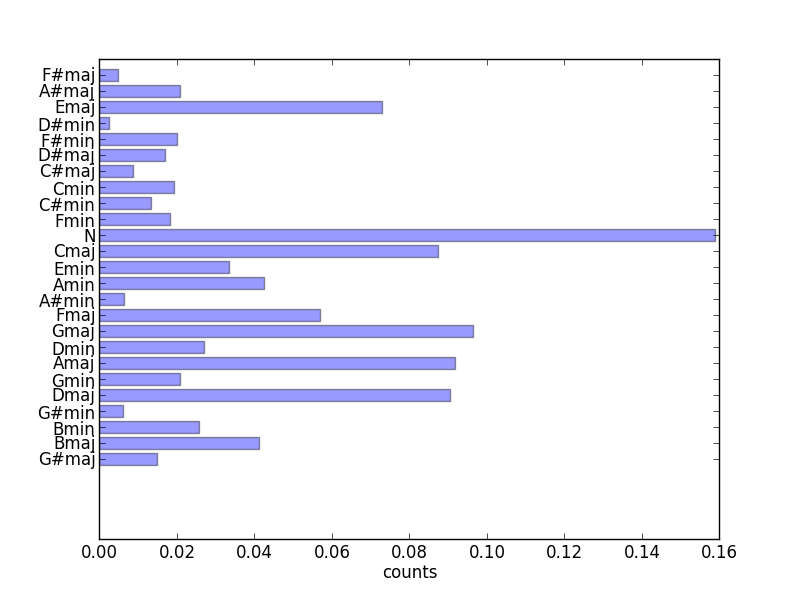
\includegraphics[width=1.0\linewidth]{chordDistrib}
\captionof{figure}{Chord distribution in our dataset}
\end{center}

}










%----------------------------------------------------------------------------------------
%	MATERIALS AND METHODS
%----------------------------------------------------------------------------------------

\headerbox{Proposed Methods}{name=method,column=1,span=2}{ % This block's bottom aligns with the bottom of the conclusion block
\begin{multicols}{2}
In this work, we investigate Deep Networks (DNs) for
learning high-level and more representative features in the
context of chord detection, effectively replacing the widely
used pitch chroma intermediate representation. And feed the features into post classifiers to get the final results. The whole system is shown as below.

\begin{center}
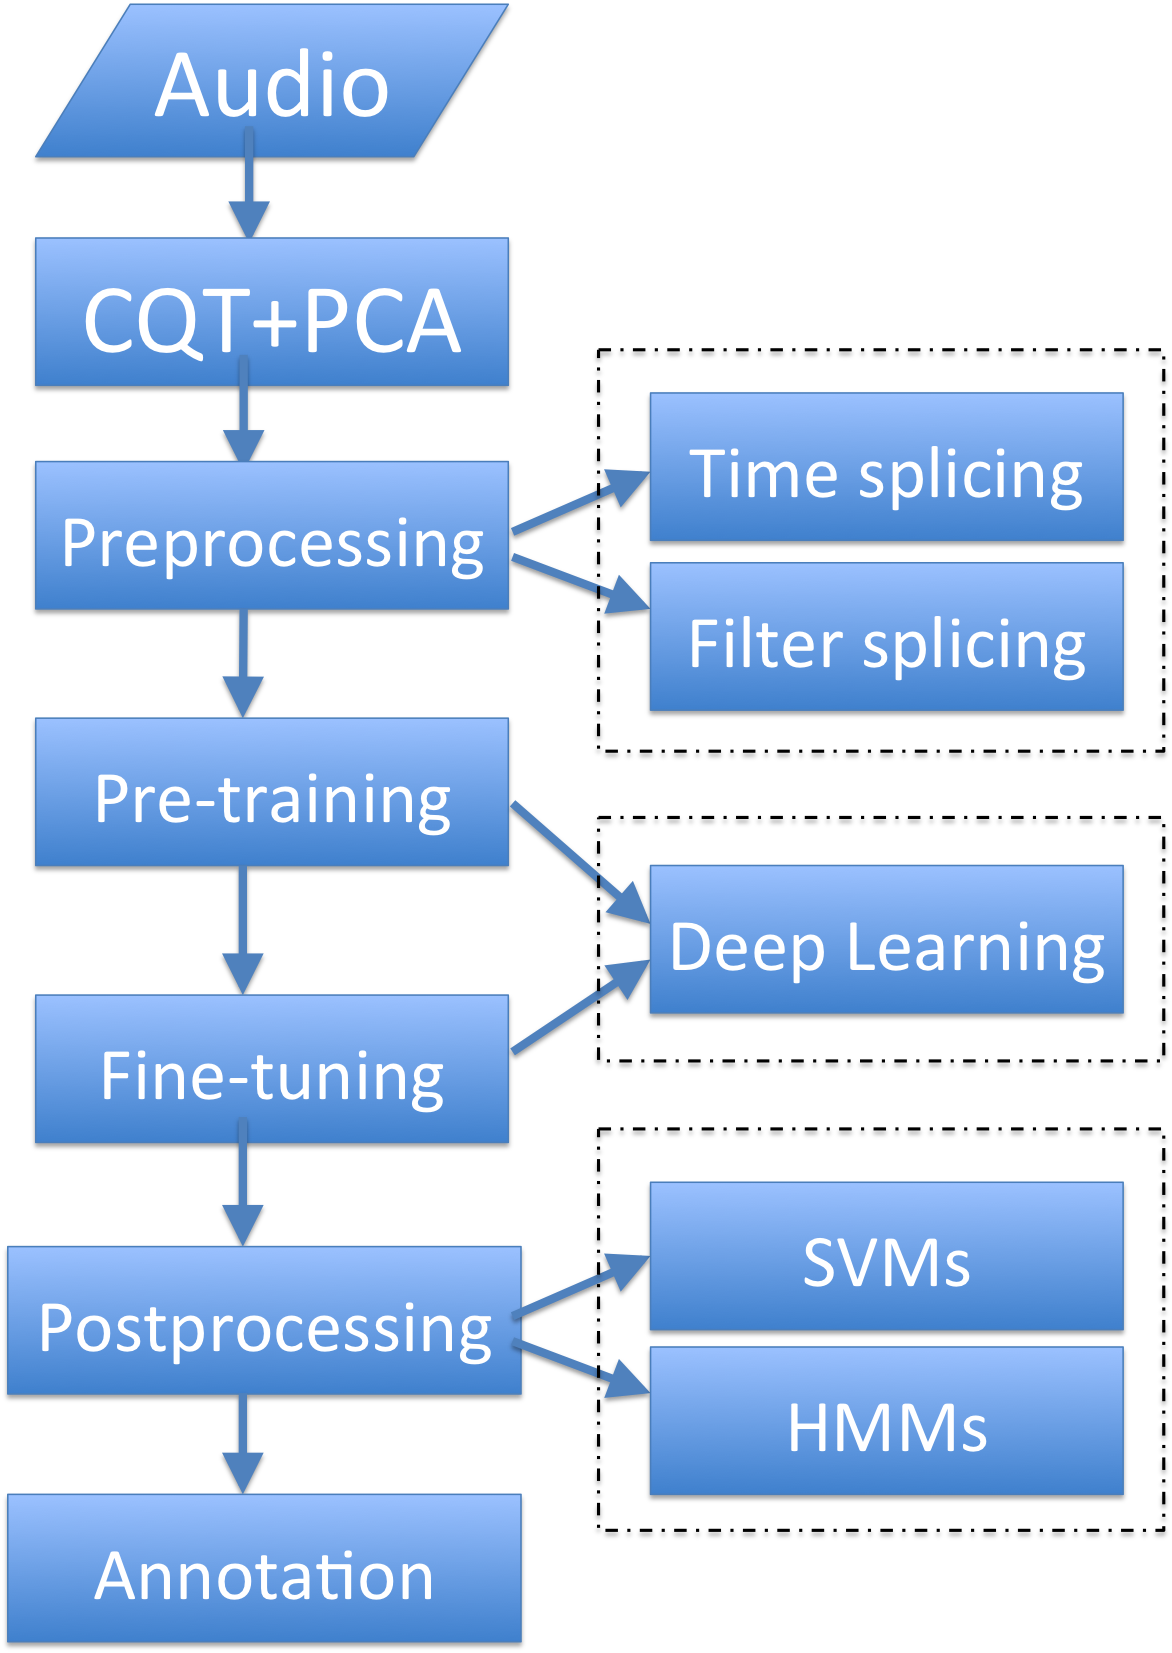
\includegraphics[width=0.60\linewidth]{flowchart}
\captionof{figure}{The flow chart of the system}
\end{center}


For pre-processing, we employ both time splicing and "convolution" (spliced filters) methods. 
\begin{itemize}\compresslist
\item Time splicing is to simply join several adjacent frames into a "super" frame
\item The "convolution" is to use a set of heuristic templates to convolve with the input frames and splice the results together, followed by an optional pooling operation.
\end{itemize}
An illustration of the convolution method is shown in the following figures: 


\begin{center}
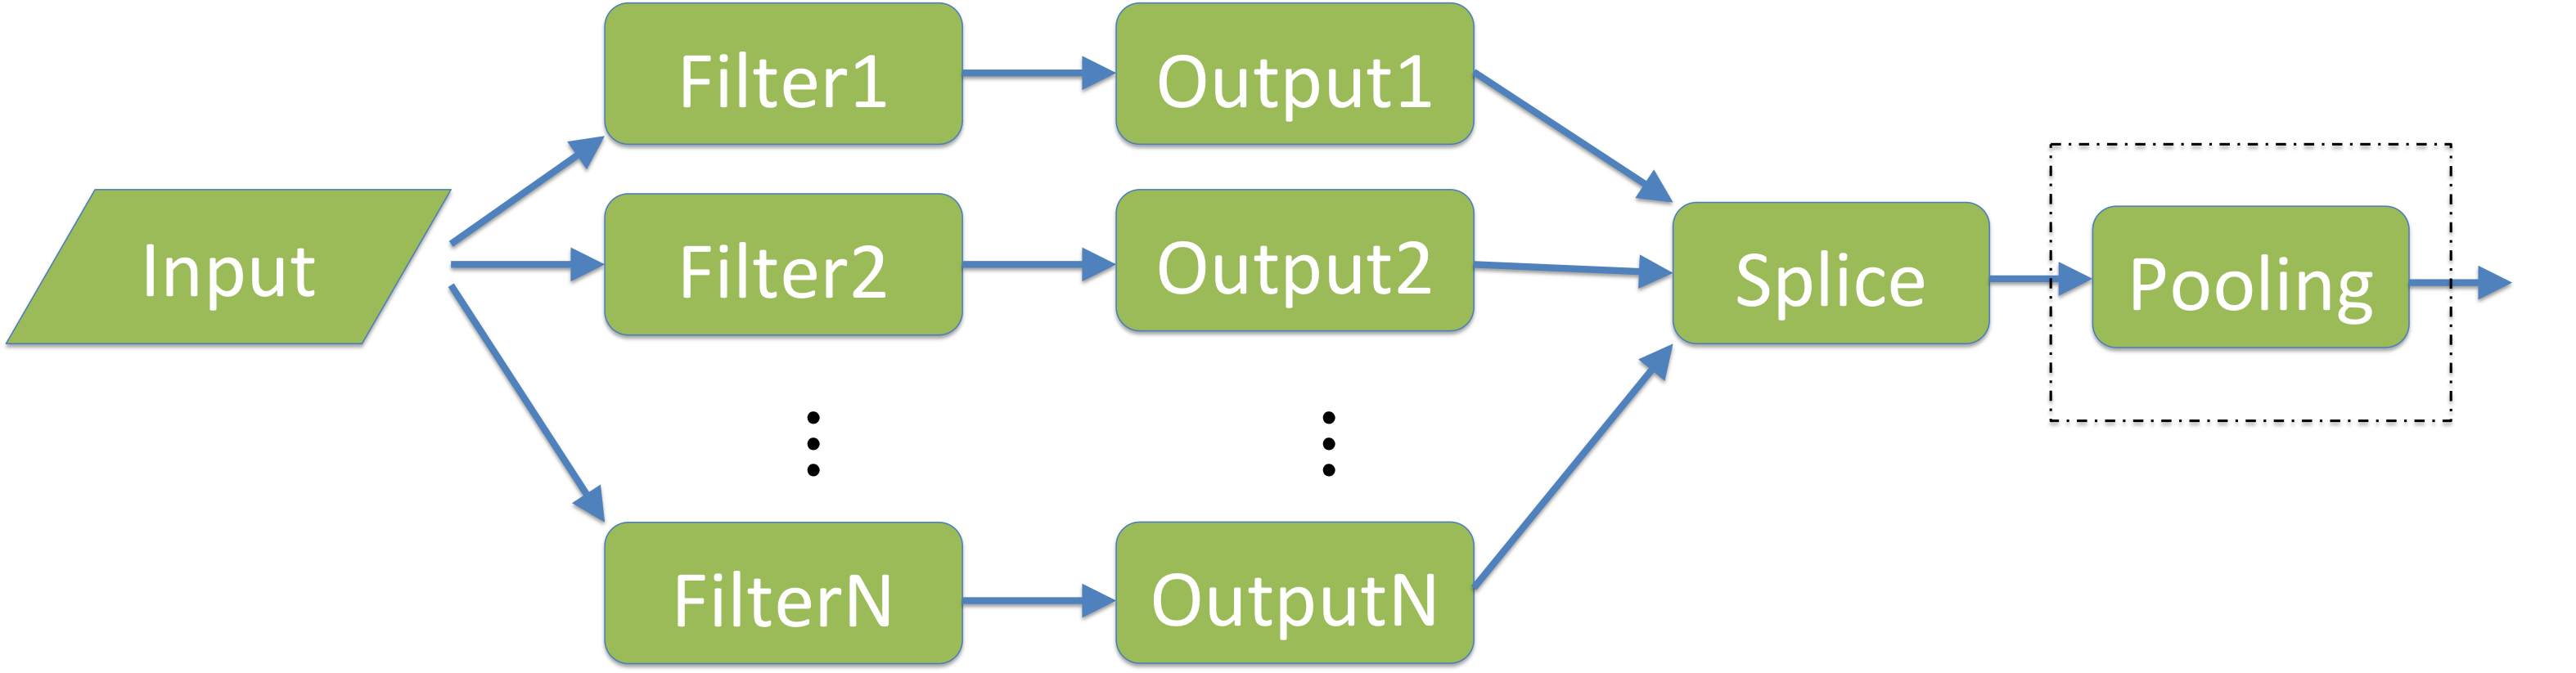
\includegraphics[width=1.0\linewidth]{CNN.png}
\captionof{figure}{Spliced filters illustration}
\end{center}

For networks architectures we compare bottleneck and the common ones; 
\begin{center}
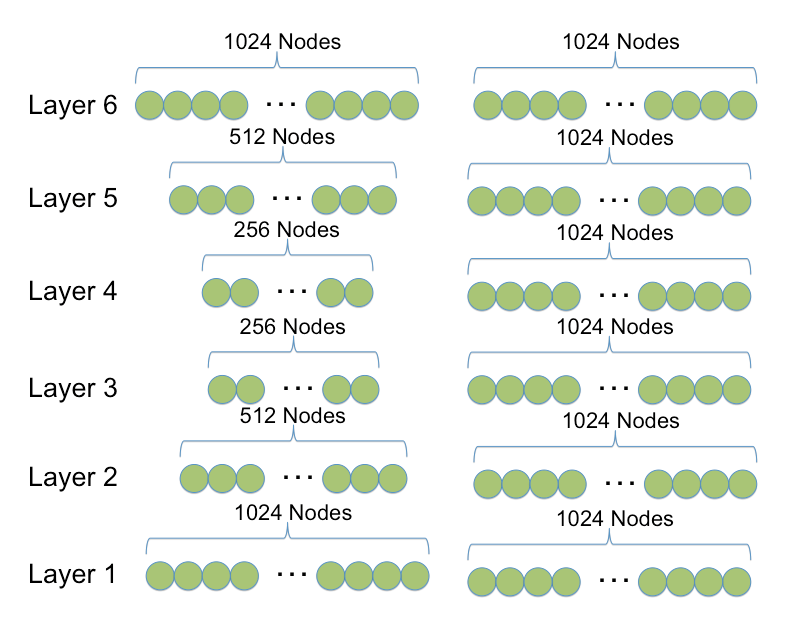
\includegraphics[width=0.9\linewidth]{arch.png}
\captionof{figure}{Architectures of bottleneck and common networks}
\end{center}

\end{multicols}
}

%----------------------------------------------------------------------------------------
%	RESULTS 1
%----------------------------------------------------------------------------------------

\headerbox{Results}{name=results,column=1,span=2,below=method}{

\begin{multicols}{2}
%\vspace{1em}
\begin{itemize}\compresslist
\item Three different post classifiers are compared. The Weighted Chord Symbol Recall (WCSR) are used to evaluate the system.
\item Both architectures is evaluated in comparison. WCSR computed on the training
set is reported as well. Different pre-processing methods are applied respectively.

\end{itemize}

%\end{multicols}
\begin{center}
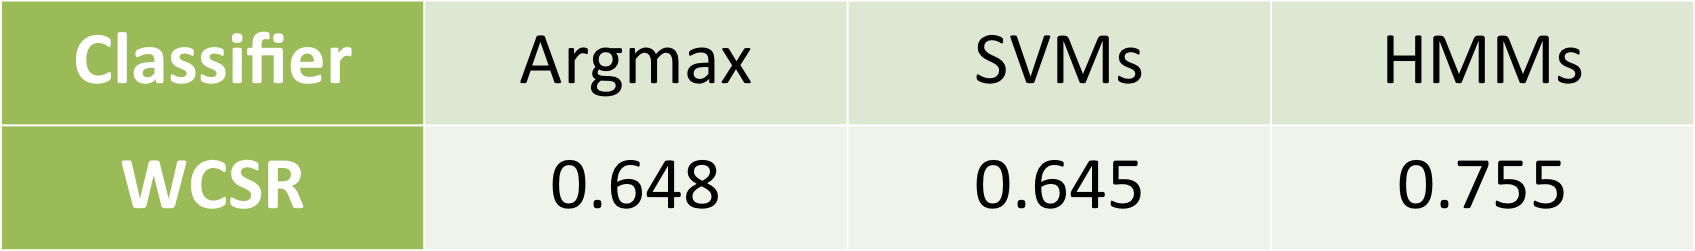
\includegraphics[width=0.8\linewidth]{post-classifier}
\captionof{figure}{Results using different post-classifiers}
\end{center}

\begin{center}
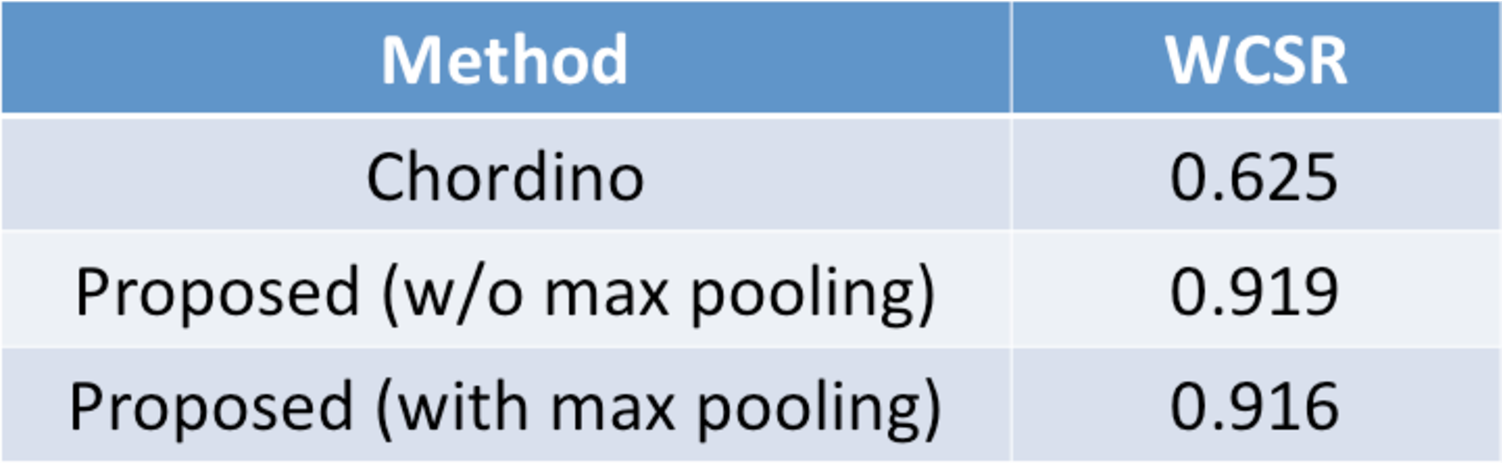
\includegraphics[width=0.8\linewidth]{final}
\captionof{figure}{Final results}
\end{center}
%------------------------------------------------

%\begin{multicols}{1}
%\vspace{1em}

 
%The bottleneck
%architecture gives significantly better results (p = 0.023)
%on the test set.
\begin{itemize}\compresslist
\item Finally, we compare our system with
Chordino\cite{mauch2010approximate} under the default settings based on our
dataset.
\end{itemize}
\begin{center}
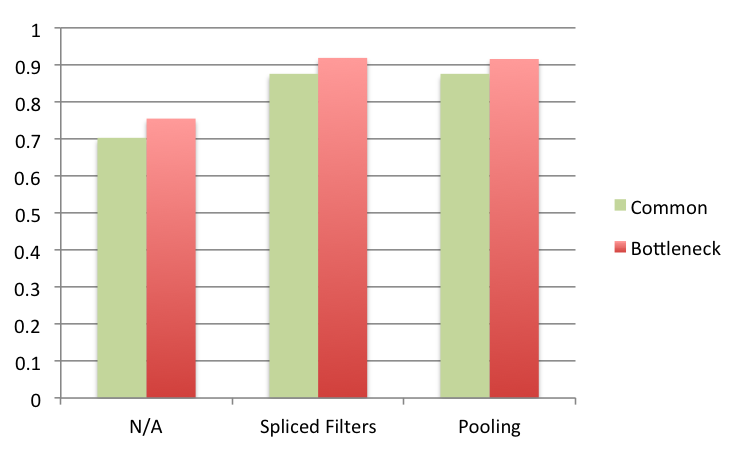
\includegraphics[width=1\linewidth]{architecture}
\captionof{figure}{Results using different architectures}
\end{center}



\end{multicols}
}
%----------------------------------------------------------------------------------------
%	RESULTS 2
%----------------------------------------------------------------------------------------

%\headerbox{Results 2}{name=results2,column=3}{ % This block's bottom aligns with the bottom of the conclusion block
%%It seems a
%%promising choice to learn pitch class information instead of the chord classes. It will,
%%however, lead to another issue: the single-label output (one
%%chord per output) will be changed into a multi-label output
%%(multiple pitches per output).
%%\begin{center}
%%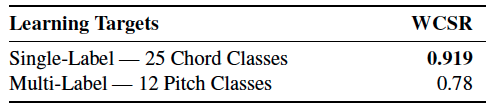
\includegraphics[width=0.8\linewidth]{multilabel.png}
%%\captionof{figure}{Comparison between training strategies }
%%\end{center}
%
%%
%Finally, we present the results of
%Chordino\cite{mauch2010approximate} with the default settings, computed on our
%dataset and compare it with our system. 
%\begin{center}
%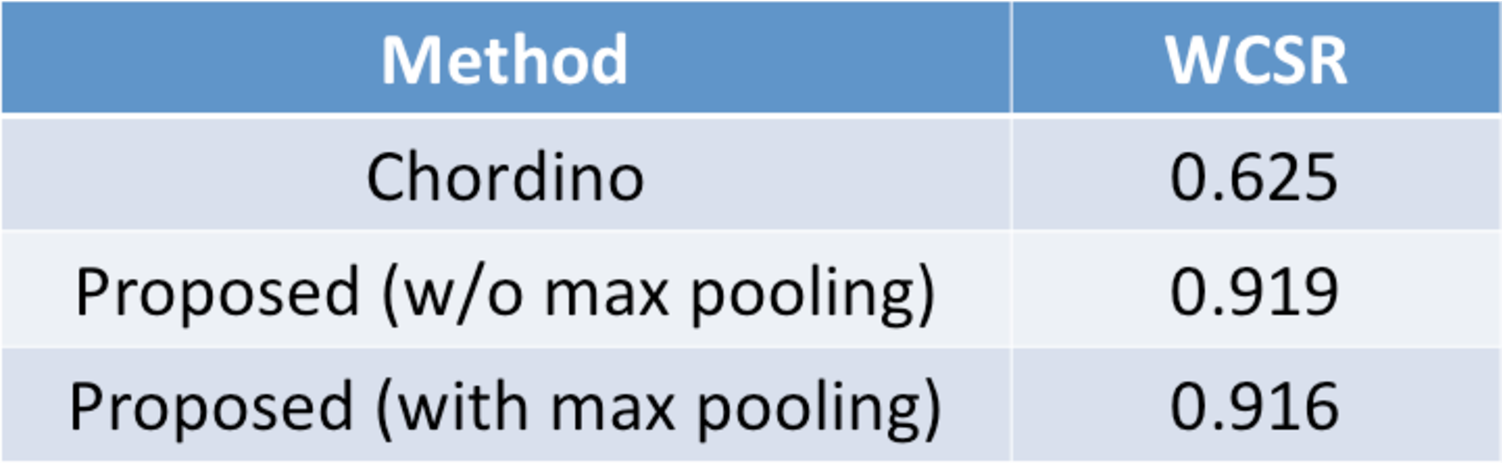
\includegraphics[width=0.9\linewidth]{final}
%\captionof{figure}{Final results}
%\end{center}
%}

%----------------------------------------------------------------------------------------
%----------------------------------------------------------------------------------------
%	CONCLUSION
%----------------------------------------------------------------------------------------

\headerbox{Conclusion}{name=conclusion,column=1,span=2,below=results,above=bottom}{



%\tikzstyle{decision} = [diamond, draw, fill=blue!20, text width=4.5em, text badly centered, node distance=2cm, inner sep=0pt]
%\tikzstyle{block} = [rectangle, draw, fill=blue!20, text width=5em, text centered, rounded corners, minimum height=4em]
%\tikzstyle{line} = [draw, -latex']
%\tikzstyle{cloud} = [draw, ellipse, fill=red!20, node distance=3cm, minimum height=2em]
%
%\begin{tikzpicture}[node distance = 2cm, auto]
%\node [block] (init) {Initialize Model};
%\node [cloud, left of=init] (Start) {Start};
%\node [cloud, right of=init] (Start2) {Start Two};
%\node [block, below of=init] (init2) {Initialize Two};
%\node [decision, below of=init2] (End) {End};
%\path [line] (init) -- (init2);
%\path [line] (init2) -- (End);
%\path [line, dashed] (Start) -- (init);
%\path [line, dashed] (Start2) -- (init);
%\path [line, dashed] (Start2) |- (init2);
%\end{tikzpicture}



%------------------------------------------------


%In this work, we presented a system which applies deep
%learning to the MIR task of automatic chord detection. Our
%model is able to learn high-level probabilistic representations
%for chords across various configurations. We have
%shown that the use of a bottleneck architecture is advantageous
%as it reduces overfitting and increases classifier performance,
%and that the choice of appropriate input filtering and
%splicing can significantly increase classifier performance.
\begin{multicols}{2}
\begin{itemize}\compresslist
\item Our
model is able to learn high-level probabilistic representations
for chords.
\item The use of a bottleneck architecture is advantageous
as it reduces overfitting and significantly increases classifier performance (p = 0.023).
\item HMMs fits the task better than the static classifiers. 
\item The choice of appropriate filtering and
splicing can significantly influence the performance.
\item The pooling operation is preferable because it reduce the system complexity without sacrificing the performance. 
\end{itemize}
\end{multicols}
%
}

%----------------------------------------------------------------------------------------
%	REFERENCES
%----------------------------------------------------------------------------------------

\headerbox{References}{name=references,column=0,below=dataset}{

\renewcommand{\section}[2]{\vskip 0.05em} % Get rid of the default "References" section title
\nocite{*} % Insert publications even if they are not cited in the poster
\small{ % Reduce the font size in this block
\bibliographystyle{unsrt}
\bibliography{conference_poster_4} % Use sample.bib as the bibliography file
}}

%----------------------------------------------------------------------------------------
%	FUTURE RESEARCH
%----------------------------------------------------------------------------------------

%\headerbox{Future Research}{name=futureresearch,column=2,below=results}{ % This block is as tall as the references block
%
%
%Learning a pitch class vector instead of chord likelihood
%with multi-label learning would allow the deep networks be independent of the number of chords to be detected. 
%
%}

%----------------------------------------------------------------------------------------
%	CONTACT INFORMATION
%----------------------------------------------------------------------------------------

\headerbox{Contact Information}{name=contact,column=0,below=references,above=bottom}{ % This block is as tall as the references block

\begin{description}\compresslist
%\item[Web] gtcmt.gatech.edu/research/music-informatics
\item[Email] {xzhou89, alexander.lerch}@gatech.edu
\item[Phone] +1 (404) 398 7794
\end{description}
}


\end{poster}

\end{document}